
%------------------------------------------------

\section{Binomial distribution}
\label{exer:binomial_distr}

\subsection{Generate binomial variables}

\begin{enumerate}
		\marginnote{Do not use any predefined method for the binomial or factorial.}
	\item Compute the distribution of binomial variables $k_{i}$ with $n = 150$ and $pi = \{ 0.1, 0.3, 0.5, 0.7, 0.9 \}$.
	\item Plot them all together.
	\item Repeat for $n = 500$.
\end{enumerate}

\subsection{Hints for the solution}

Compute the binomial coefficient using $a = \exp( \ln(a) )$, and simplify the terms that cancel out:

\begin{equation}
	\mathrm{BinomialCoeff}(n, k) 
	= \exp \left[ \sum_{i = n - k + 1}^{n}{\ln(i)} - \sum_{i = 2}^{k}{\ln(i)} \right]
\end{equation}

Compute the Bernoulli term with $a = \exp( \ln(a) )$ to avoid numerical problems in the situation that $p$ is small and $(1 - p)$ large, or viceversa:

\begin{equation}
	p^{k}(1 - p)^{n - k} = \exp \left[ k \ln(p) + (n - k) \ln(1 - p) \right]
\end{equation}

(Figure~\ref{fig:binomial_distr_n_150} and~\ref{fig:binomial_distr_n_500})

\begin{figure}
	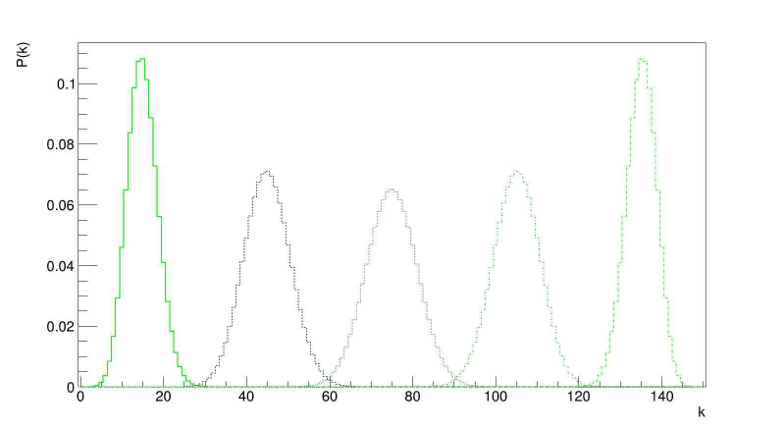
\includegraphics{exercise/binomial_distr_n_150.png}
	\caption[Binomial distribution ($n = 150$).][6pt]{Binomial distribution ($n = 150$).}
	\label{fig:binomial_distr_n_150}
\end{figure}

\begin{figure}
	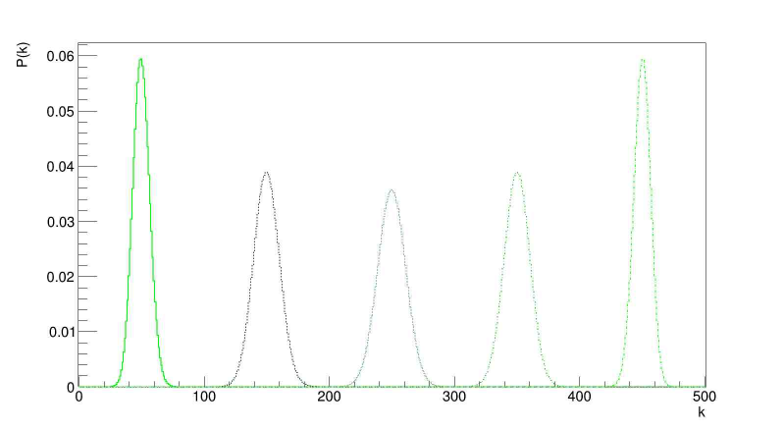
\includegraphics{exercise/binomial_distr_n_500.png}
	\caption[Binomial distribution ($n = 500$).][6pt]{Binomial distribution ($n = 500$).}
	\label{fig:binomial_distr_n_500}
\end{figure}

($\hookleftarrow$ \ref{subsec:binomial_distr})
